% 第1章第3节：连续函数空间（一致范数与一致收敛；输入域与范数的改变）。

\section{连续函数空间}
\label{sec:fs-continuous}

上一节的定义需要一个完整的例子来落地。本节固定紧区间上的连续函数，配上最大偏差范数，证明得到的是Banach空间。这是最接近一元分析经验的函数空间；随后我们改变输入域和范数，看哪些结论需要重新检查。

\subsection{一致范数与一致收敛}
\label{sec:fs-uniform-norm}

在$C([a,b])$上定义
\begin{equation}
 \|f\|_\infty=\sup_{x\in[a,b]}|f(x)|,
 \label{eq:fs-uniform-norm}
\end{equation}
称为\term{一致范数}（uniform norm）或上确界范数。$|f|$是紧集上的连续函数，由最值定理（定理~\ref{thm:metric-extreme-value}）取到最大值，所以上确界有限，而且实际上是最大值。

范数公理逐条成立。若$\|f\|_\infty=0$，则每一点$|f(x)|\leq0$，$f=0$。齐次性来自$|cf(x)|=|c||f(x)|$在每点成立后取上确界。对三角不等式，每个$x$处都有$|f(x)+g(x)|\leq|f(x)|+|g(x)|\leq\|f\|_\infty+\|g\|_\infty$，右边与$x$无关，对$x$取上确界即得$\|f+g\|_\infty\leq\|f\|_\infty+\|g\|_\infty$。

\paragraph{范数收敛就是一致收敛}
把$\|f_n-f\|_\infty\to0$按定义展开：对每个$\varepsilon>0$存在$N$，使$n\geq N$时$\sup_x|f_n(x)-f(x)|\leq\varepsilon$，即对\emph{所有}$x$同时有$|f_n(x)-f(x)|\leq\varepsilon$。这正是一致收敛：同一个$N$管住全部输入位置。逐点收敛与一致收敛的区别及$x^n$的经典例子，可参考\BookChapterRef{chap:limits-continuity}{卷一“极限与连续”章}。

图~\ref{fig:fs-uniform-tube}给出了几何图像。$\|f_n-f\|_\infty\leq\varepsilon$等价于$f_n$的整条曲线落在以$f$为中心、上下宽$\varepsilon$的带子里，如(a)所示。(b)中的$x^n$在$[0,1)$上逐点趋于$0$，但每条曲线在靠近$x=1$处都会越出零函数周围的带子：$x^4$在$x=0.15^{1/4}\approx0.62$处越出，$x^{12}$推迟到$x=0.15^{1/12}\approx0.85$，越出点随$n$右移，却始终存在。

\begin{figure}[!htb]
  \centering
  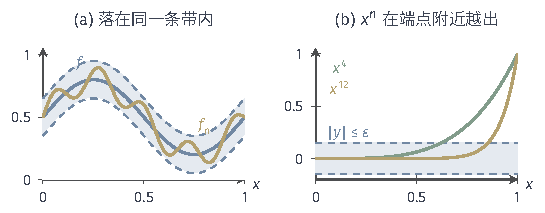
\includegraphics[width=92.2mm]{figures/02-abstract-mathematics/03-function-spaces/tikz/c1-uniform-tube/figure.pdf}
  \caption{一致范数的几何意义。(a)$f(x)=0.5+0.3\sin(2\pi x)$周围宽$\varepsilon=0.15$的带子（浅蓝），$f_n=f+0.1\sin(9\pi x)$整条曲线都在带内，所以$\|f_n-f\|_\infty=0.1\leq\varepsilon$。(b)零函数周围同样宽的带子；$x^4$与$x^{12}$在靠近$x=1$处越出，因为$\|x^n\|_\infty=1$对每个$n$都成立。}
  \label{fig:fs-uniform-tube}
\end{figure}

用一致范数可以把“$x^n$在$[0,1]$上不一致收敛”写成一个具体的数。取$m=2n$，令$t=x^n\in[0,1]$，则
\[
 \|x^n-x^{2n}\|_\infty=\max_{t\in[0,1]}(t-t^2)=\frac14,
\]
最大值在$t=\tfrac12$处取到。这个值不随$n$减小，所以$(x^n)$在$C([0,1])$中连Cauchy列都不是。若把区间缩小到$[0,\tfrac12]$，则$\|x^n\|_\infty=2^{-n}\to0$，一致收敛到零函数。

\paragraph{连续函数空间的完备性}
一致范数下的极限能否留在$C([a,b])$中，是下面这个定理的内容。它的证明包含三个步骤：先构造候选极限，再把逐点收敛加强为一致收敛，最后证明极限连续。三个步骤各有职责，不能从逐点极限直接跳到空间内的收敛。

\begin{theorem}[连续函数空间的完备性]
\label{thm:fs-continuous-complete}
$(C([a,b]),\|\cdot\|_\infty)$是Banach空间。
\end{theorem}

\begin{proof}
设$(f_n)$是一致范数下的Cauchy列。

第一步，逐点构造候选极限。固定$x\in[a,b]$，有$|f_n(x)-f_m(x)|\leq\|f_n-f_m\|_\infty$，所以实数列$(f_n(x))$是Cauchy列。由实数的完备性，它收敛，记极限为$f(x)$。这样得到一个函数$f:[a,b]\to\mathbb R$，但目前只知道$f_n$逐点收敛到它。

第二步，把共同误差界传给极限。给定$\varepsilon>0$，取$N$使$m,n\geq N$时$\|f_n-f_m\|_\infty<\varepsilon$。固定$x$与$n\geq N$，在$|f_n(x)-f_m(x)|<\varepsilon$中令$m\to\infty$，得$|f_n(x)-f(x)|\leq\varepsilon$。这个界与$x$无关，所以$\sup_x|f_n(x)-f(x)|\leq\varepsilon$对所有$n\geq N$成立，即$f_n$一致收敛到$f$。

第三步，证明极限连续。固定$x_0$与$\varepsilon>0$。由第二步取$N$使$\sup_x|f_N(x)-f(x)|<\varepsilon/3$；$f_N$连续，存在$\delta>0$使$|x-x_0|<\delta$时$|f_N(x)-f_N(x_0)|<\varepsilon/3$。对这样的$x$，
\[
 |f(x)-f(x_0)|\leq|f(x)-f_N(x)|+|f_N(x)-f_N(x_0)|+|f_N(x_0)-f(x_0)|<\varepsilon .
\]
所以$f$在$x_0$连续。$x_0$任意，$f\in C([a,b])$；结合第二步，$\|f_n-f\|_\infty\to0$。
\end{proof}

第三步中的“三项误差分解”值得记住：两端的项靠一致收敛统一控制，中间一项靠某个固定的$f_N$的连续性控制。若只有逐点收敛，两端的项无法对邻域内所有$x$同时变小，$x^n$在$[0,1]$上的不连续极限就是例子。

\subsection{输入域与范数的改变}
\label{sec:fs-domain-norm-change}

定理~\ref{thm:fs-continuous-complete}用到了输入域和范数的两项性质：上确界有限，以及一致收敛保持连续。改变输入域或范数时，需要检查的正是这两点。

\paragraph{紧度量空间上的连续函数}
把$[a,b]$换成任意紧度量空间$K$，定义$C(K)$为$K$上的实连续函数，配以$\|f\|_\infty=\sup_{x\in K}|f(x)|$。最值定理在紧度量空间上成立，所以上确界有限；完备性证明的三个步骤只用到实数完备性与度量空间中连续的定义，原样适用。因此$C(K)$也是Banach空间。当$K=\{1,\ldots,n\}$是有限集（任意度量下都紧）时，$C(K)$就是$\mathbb R^n$配最大分量范数。

\paragraph{非紧域与有界连续函数}
在非紧域上，连续函数可能无界：$\mathbb R$上的$f(x)=x$的上确界为$+\infty$，一致“范数”不再是实数。此时改用有界连续函数空间
\[
 C_b(X)=\{f:X\to\mathbb R\ \text{连续}:\ \sup_{x\in X}|f(x)|<\infty\},
\]
配以同样的上确界范数。完备性证明前两步不变。第二步得到的一致误差界还说明极限有界：取定$N$后，对每个$x$都有$|f(x)|\leq\|f_N\|_\infty+\varepsilon$。第三步不依赖紧性。故$C_b(X)$对任意度量空间$X$都是Banach空间。

非紧域上会出现紧区间上没有的现象。在$C_b(\mathbb R)$中取移动的三角形$f_n(x)=\max(0,1-|x-n|)$：每个固定的$x$在$n>|x|+1$后都满足$f_n(x)=0$，所以$f_n$逐点趋于零；但三角形的峰高始终为$1$，$\|f_n\|_\infty=1$，序列不一致收敛。质量没有消失，只是移到了无穷远处。

\paragraph{局部一致收敛}
有些序列在每个有界范围内都一致收敛，在整条实轴上却不收敛。$f_n(x)=x/n$不在$C_b(\mathbb R)$中，但对每个$R>0$，$\sup_{|x|\leq R}|f_n(x)|=R/n\to0$。这种“在每个紧集上一致收敛”称为局部一致收敛，它由一族上确界$\sup_{|x|\leq R}|\cdot|$共同描述，不是单个范数给出的收敛。这类由一族半范数定义的空间不在本章展开；我们只需记住：一致范数关注整个输入域，局部一致收敛只关注每个紧集。

\paragraph{改换范数后的同一集合}
回到同一个集合$C([-1,1])$。在一致范数下它是Banach空间（定理~\ref{thm:fs-continuous-complete}）；换成平方积分范数$\|\cdot\|_2$，第~\ref{sec:fs-banach}小节的斜坡列是Cauchy列却没有连续极限，空间不完备。集合没有变，变的是“接近”的标准。斜坡列在一致范数下不是Cauchy列：对$m>n$，在$x=1/m$处$g_m=1$而$g_n=n/m$，所以$\|g_n-g_m\|_\infty\geq1-n/m$，取$m=2n$即得$\|g_n-g_{2n}\|_\infty\geq\tfrac12$。

平方积分误差关心的是整体偏差，自然的极限是阶跃函数，而它在$0$处的值无关紧要。要让这样的极限有处可去，就需要把成员扩大到可测函数，并且忽略零测集上的差别。这就是下一节积分函数空间的出发点。
